\section{PADAR as observer-field dynamics}\label{sec:attention-padar}

\begin{definition}[Attention]
Attention is retained field/observer orientation on returned duon current.
\end{definition}

The field attention vector was defined in Section~\ref{sec:duonic-pressure-inertia} as pressure-weighted lead--lag relation motion:
\[
A_{\mathcal F}^{(q)}(\partial F,\omega)=
\sum_{e\in\mathcal F(\partial F,\omega)}
p^D_e(\partial F,\omega)r^{(q)}_e(\omega).
\]
It is pressure-weighted relational motion carried by PADAR.

\begin{figure}[H]
\centering
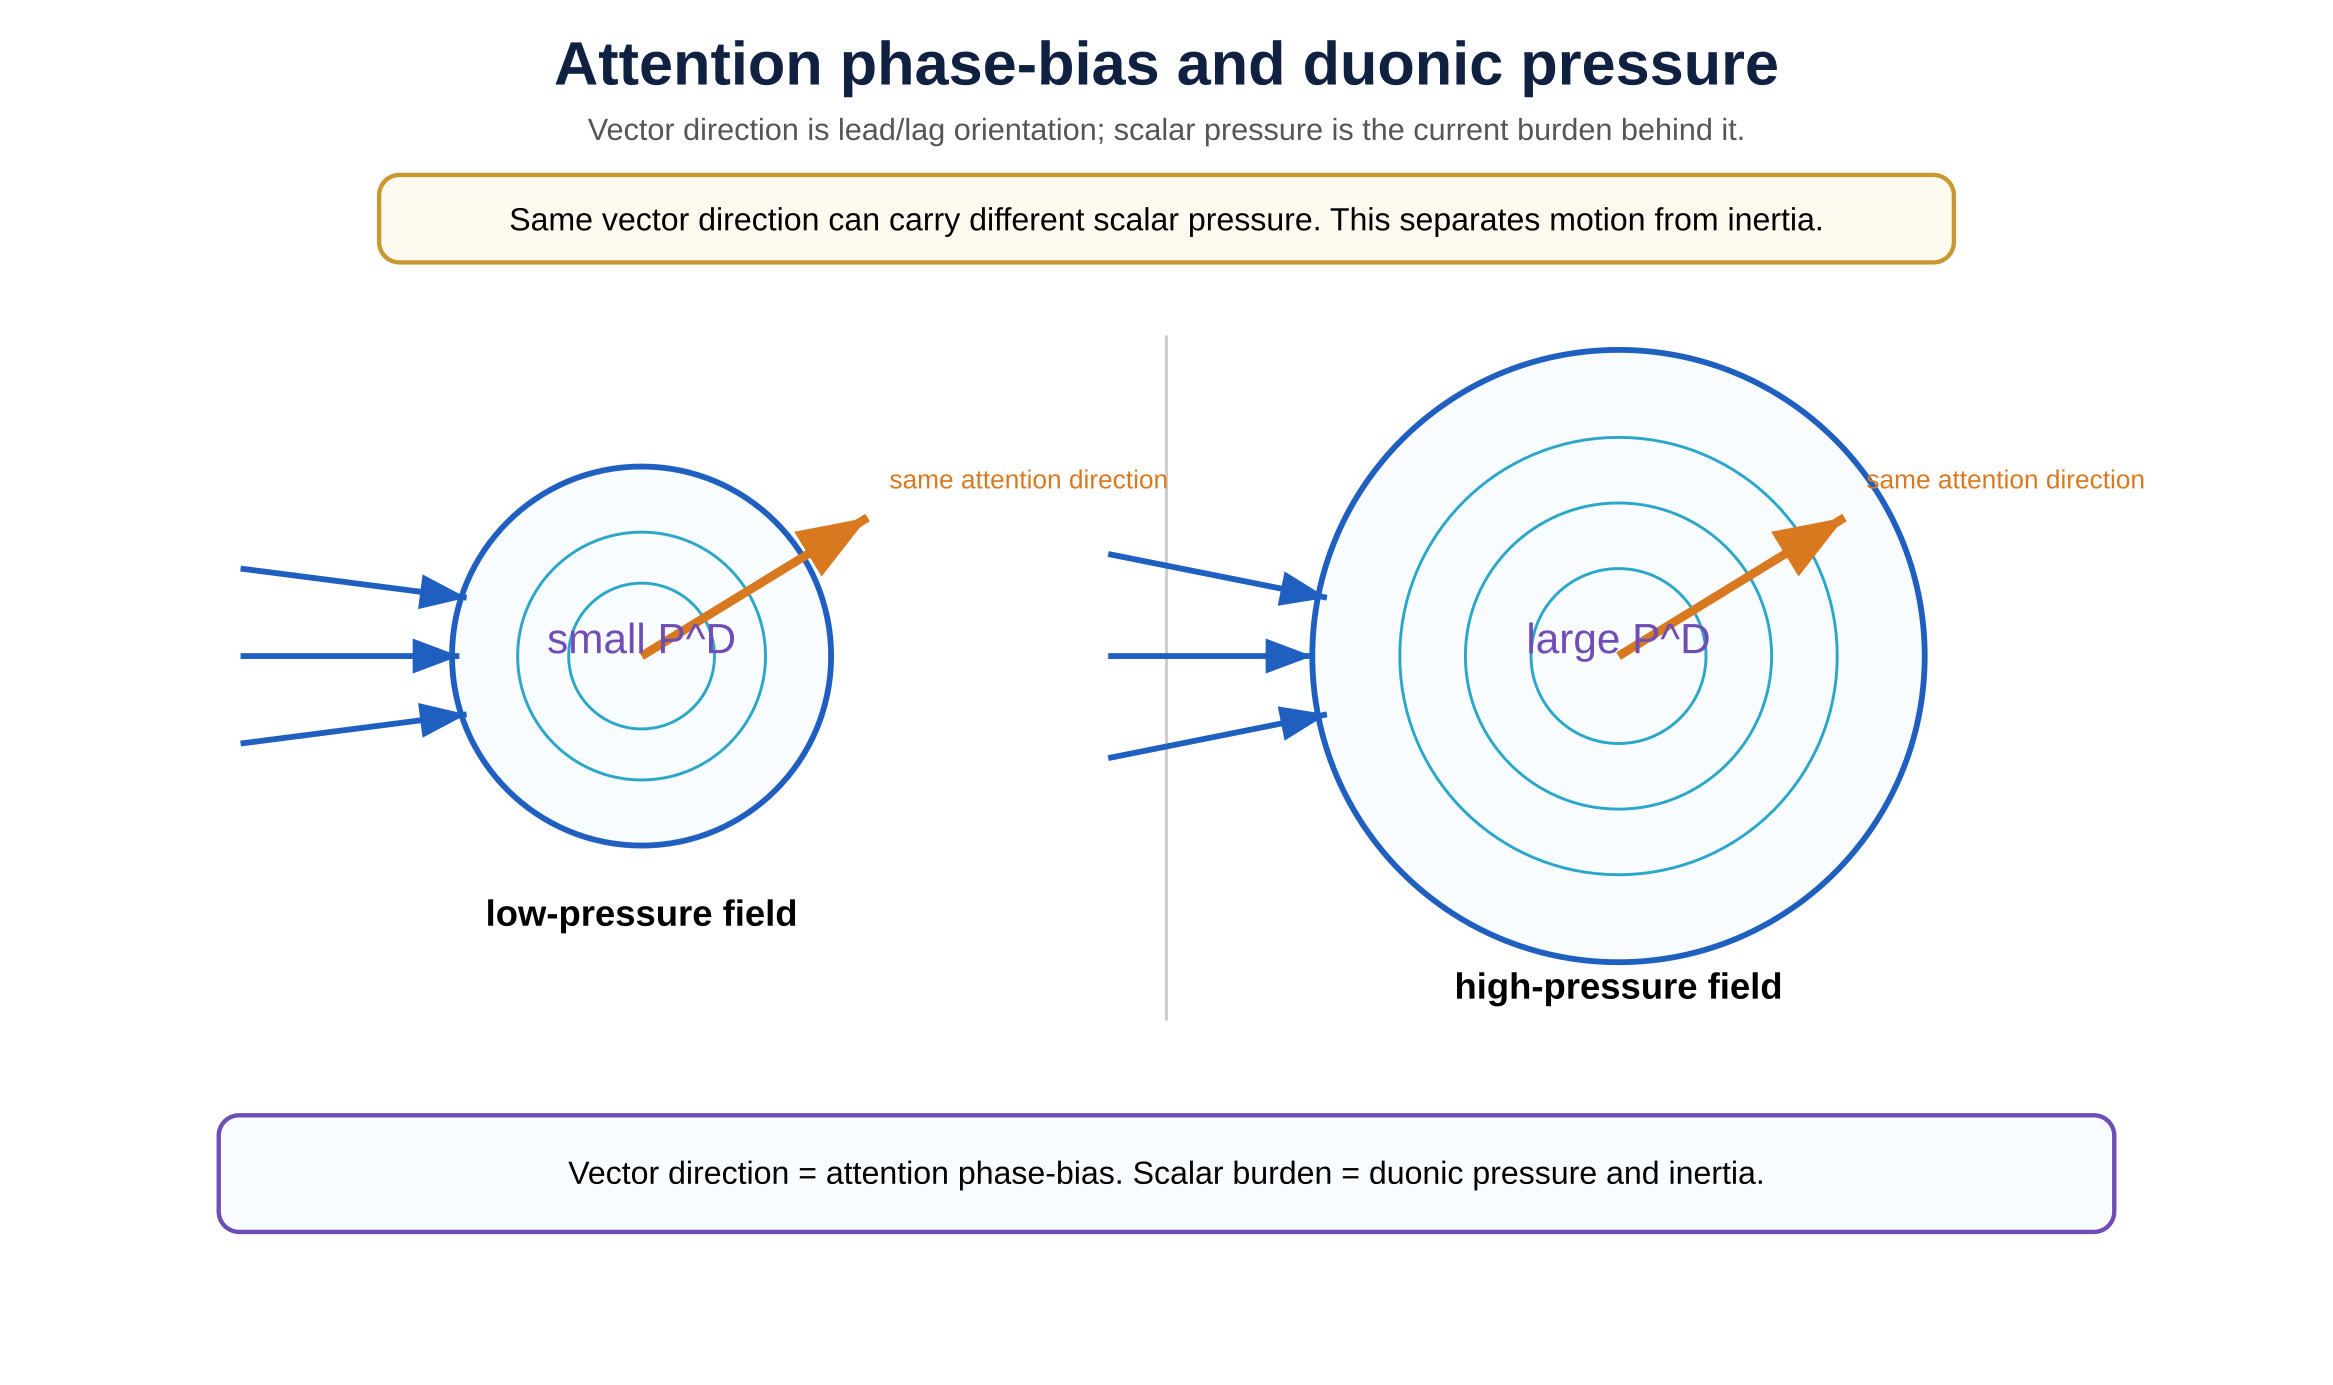
\includegraphics[width=0.98\linewidth]{figures_jpg/v39_attention_phase_bias_pressure.jpg}
\caption{Field attention vector and duonic pressure. The normalized orientation gives direction; duonic pressure supplies retained burden; the field attention vector combines them as pressure-weighted relation motion.}
\label{fig:v39-attention-pressure}
\end{figure}

\begin{definition}[ADAR]
ADAR is one local returned-current channel:
\[
\ADAR_e=(A_e,D_e,R^{\mathrm{asym}}_e).
\]
Here \(A_e\) is retained attention orientation, \(D_e\) is retained cut-return duration, and \(R^{\mathrm{asym}}_e\) is asymmetric reflection. RCD is the local name for the duration/reflection coupling
\[
\RCD_e = D_e\leftrightarrow R^{\mathrm{asym}}_e
\]
inside the ADAR channel.
\end{definition}

\begin{definition}[PADAR]
PADAR is Poly Attention--Duration--Asymmetric Reflection: the field consequence of rebalancing cut-running asymmetry through attention, duration, and asymmetric reflection. It records how the observer-field retains attention orientation, return duration, pressure, and asymmetric reflection across simultaneous returned-current channels:
\[
\PADAR_{\mathcal F}(\partial F,\omega)=
\{\ADAR_e(\partial F,\omega)\}_{e\in\mathcal F(\partial F,\omega)}.
\]
\end{definition}


\subsection{Poly boundary principle}\label{subsec:poly-boundary-principle}
The fixed-scope field count is defined in Section~\ref{sec:field-count-padar-scope}. In that scope, \(\mathcal F_{\mathcal B}\), \(n_F(\mathcal B)\), returned-current channels \(\ADAR_{i\leftarrow j}\), and \(K_{\partial F}(\mathcal B)\) supply the finite poly argument of PADAR.

The field attention vector is carried by PADAR dynamics:
\[
A_{\mathcal F}^{(q)}(\partial F,\omega)
\in
\PADAR_{\mathcal F}(\partial F,\omega).
\]
Component views may project this vector, but the vector itself records pressure-weighted field relational motion.
